%update: Dec 20 wrote more. 

\begin{savequote}[75mm] 
In three words I can sum up everything I've learned about life: it goes on.
\qauthor{Robert Frost} 
\end{savequote}

\chapter{Conclusions and Future Perspectives}

\newthought{In} summary, probing technique is applied to \emph{in situ} TEM.

\section{Conclusions}
%chapter 3
In chapter 3, a direct and powerful {\em in situ} HRTEM technique to construct individual axial nanowire junctions -- which perfectly highlighting the popular {\em nanoarchitectonics} concept -- has been for the first time realized. {\em In situ} HRTEM and in-tandem crystallography characterizations and optoelectronic behavior tests unveal the photosensing properties of the single-crystalline axial CdS/p-Si nanowire junctions. The junctions exhibit good selectivity toward the light frequencies higher than those of the yellow range. The junctions possess a specific photocurrent saturation effect; this could be utilized in low-consumption light intensity sensing and integrated tunable voltage-driven applications thanks to the corresponding current limitations and excellent tolerance toward possibly unreliable and unstable bias. Clearly, the present nanoarchitectonics-based approach employing in situ structural design and measurements gives a strong motivation for establishing new operational principles of single crystal nano-devices. Furthermore, it is also envisaged that the near-field scanning technique could be also integrated within the designed system for even deeper understanding of the exciting nanoscale optoelectronic phenomena.\cite{Gu2005,Xiang2012}.
%chapter 4
In chapter 4, we designed a "phase-transformation" route to fabricate a doped graphene-phosphorous structures with layered morphologies in which very thin amorphous red P layers are formed within flexible and conductive N-doped graphene frameworks. Advantages of such SIB anode designs have been proved experimentally, they are namely: \\
(1) By spreading amorphous P to form a thin P layer on the doped graphene instead of crystalline P nanoparticles, the P@GN anode shows ultrastable efficiency (0.002\% decay per cycle from 2nd to 350th cycle) and excellent rate capability (809 mAh/g at 1500 mA/g); \\
(2) The expected P-C chemical bonds are detected, which firmly anchor GN and P layers; \\
(3) In situ HRTEM experiments on a prototype P@GN-based nanobattery device further verified its ultrastable performance and high capacity of P@GN entirely sustained during sodiation.\\
Finally, DFT calculations reveal that doping sites can enhance the interactions between Na and graphene surface, leading to ultrafast sodium energy storage. Our work demonstrates that the designed flexible amorphous P@N-doped graphene structure prepared from a "phase-transformation" approach can greatly improve the cycling and rate performances for future sodium storage. 
%chapter 5
Chapter 5 is a report on opto-mechano-electrical tripling phenomenon under in situ observation and measurements of photocurrents in ZnO nanowires in real time and under the highest spatial resolution natural for a high-resolution TEM instrument. By comparing nicely resolved photocurrent spectra of individual ZnO nanowires under bending deformations splitting of photocurrent spectra is observed. The shifts of photocurrent peaks are directly dependent on the bending strains. The red and blue shifts of ZnO photocurrent peaks under bending are confirmed to be directly related to the splitting of levels in the valence band at $\Gamma$ point. DFTB simulations have an excellent agreement with the experimental data. The discovered splitting effect under specially designed ZnO nanowire photocurrent spectroscopy provides an important information for flexible optoelectronics and piezo-phototronics, for example, for strain tuned wavelength-division multiplexing and MOEMS devices, and for flexible optoelectronics where photocurrent splitting should be evaded. 
%chapter 6 
In chapter 6, we have successfully performed pioneering photocurrent measurements for elastically deformed CdS nanowires inside the HRTEM. Using in situ electrical probing and light illumination, we have characterized the electronic (dark, light-off) and optoelectronic (light-on) features of individual nanowires undergoing mechanical deformation. To make the data reliable in a view of future technological applications, a large variety of nanowires was tested, allowing for a statistical analysis of their properties. All nanostructures reveal very close photocurrent-to-dark current ratios (ON/OFF ratios) in original, bent and recovered states, with an average value of approximately 10. Photocurrent spectroscopy of several examples shows red shifts of the order of several nanometers for the photocurrent cut-off wavelength. These small shifts are likely caused by deformation, which induces variations in the band structure. By taking HRTEM images, non-uniformly distributed lattice defects were found after bending. Our experiments reveal a variety of bending-induced effects for individual nanowires, while showing that from a statistical point of view the nanowires display common features in their response to deformation, making them suitable for future flexible optoelectronic applications. 

\section{Future perspectives}
%this subsection is unnecessary
%\subsection{Look back to history to see where we are}
%Anthropologist belive that an evolution of mankind would be linked to the use of tools. \cite{lilley1948men} The acients made tools to handle things at meter scale, such as knife, wrench, scythe, sickle. Human civilization histroy is very much related to to development of tools. By updating tools, humankind are able to handle meter scale objects, and gradually a few scales different from our size. The advancement of tools development is directly determined by development of science and technology. 

%From millions of years ago, humankind started to updating tools. During prehistroy (beore 3,000 BC) and ancient age (3,000 BC to 476 AC), more and more well made stone, bronze and iron made tools came out to serve human beings for daily use -- at a scale from centimeter to hundreds of meters. In paleolithic age, people are mainly making simple tools; while in neolithic age, people are experienced with applying tools to building constructions. The capability of human beings are still restricted withing 3 scales from ourselves. It is called {\em meter-scale age}. 

%In medieval age (476 AC to 1492 AC), the development of classical optics, including the production of well-made lenses, laid the groundwork for microscopy -- the tool to reach microscale and astronomical scale. In modern age (1492 AC to 1789 AC), many revolutionary researches in optics and microscopy are associated and contributed to the fast development of physics, chemistry, biology and material science. It is called {\em micro-scale age}. 

%During the last centry, development of partical physics, theory of relativity and quantum mechanics made it possible to see nanoscale world by electron microscopy and atomic force microscopy. It is called {\em nano-scale age}.

%The important mark between each "scale age" is the invention of optical microscope and electron microscope, because the preliminary important thing to do with the scale is to see objects in that scale. The main activities at early stage of each "scale age" are development of the microscopy itself as well as observing and getting knowledge of the new world objects. The main activities at second stage of each "scale age" is the production of building blocks and applications in that scales. Only when people are very familiar with almost everything in that scale with daily used applications, then science advances might move to the next scale by the rising theories and exiting experiments. 

%After developing precised mechanics, human are able to make fine mechanics to operate small objects. The gear was able to transfer larger movement into fine movements. The ratio could be improved by the development of advanced gearing. However, it is not until recent years that people are able to reach nanometer precision on mechanics when piezoelectric motor is available. \cite{} 

%Clearly we are now in the cross road between first stage and second stage of the {\em nanoscale age}. 

\subsection{Nanoscale building blocks in future}
Although many researchers claim their nanomaterial samples are perfect and uniform, the quality is not as perfect to perform identical physical or chemical properties. In chapter 6, it is noticed that even the ratios of photo-to-dark current ratios in different states is more or less stable, the photo-to-current ratios of each nanowire is very differnt from each other. The scattered distribution of the ratios is caused by the uniform structural behavior and chemical composition. To use the nanowires in bundles is practical in some applications, while it is not practical to apply them in single nanowire devices as mass production. \\
It is expected that nanoscale building blocks can be really uniform at the nanoscale. What nanoscale building blocks to complicated nanoworld applications is the bricks to the architecture. When the synthesis of various nanoscale building blocks can be well controlled to reach identical morphology, surface and physical, chemical properties. 
Another problem is the understanding of many nanomaterials are not comprehensive. But if the materials are synthesized 

\subsection{Nanomanipulations in microscopy in future}
We are now in 2017, the age of nanotechnology, of gene eneineering, of information technology, artificial intellegence and many more. According to the history of tools, human beings are now quite new to nanometer scale. The tools we are using for the nano world are electron microscopy, atomic force microscopy, lithography, piezoelectric probing and other mechanical technologies. It is true that various nanostructures are successfully synthesized, designed electronic chips are in mass production, observations are performed at atomic resolution. However, lithography technology does not work for many other applications, microscopy has sampling limitations, mechanical technology is not mature yet to handle nanoscale building blocks easily. 

\begin{figure}  
\centering
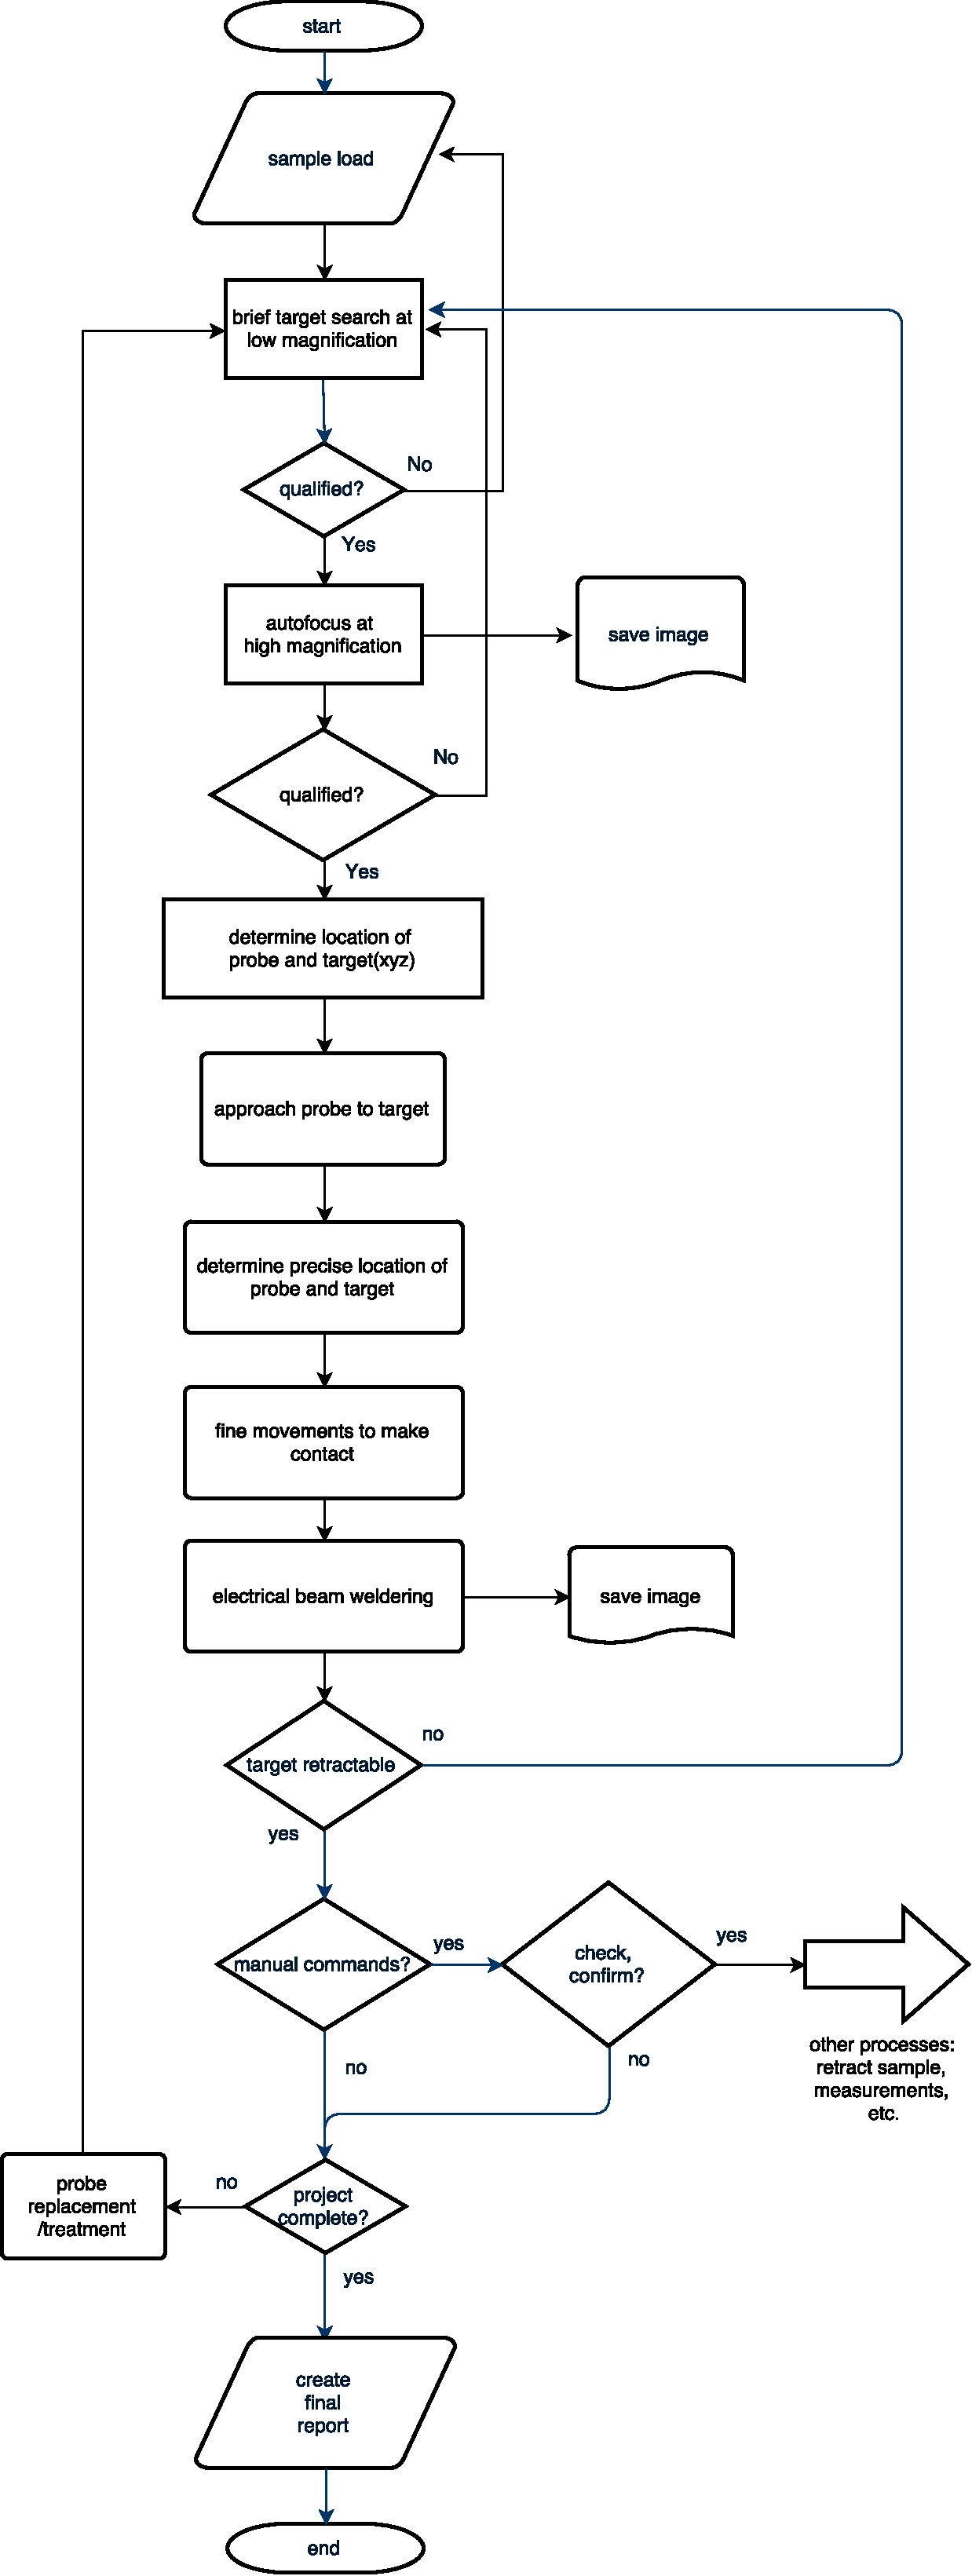
\includegraphics[width=200pt]{figures/aifornanomanipulation}
\caption[AI for Nanomanipulation]
{The workflow for nanoscale manipulations by automation.
\label{fig:7_aiworkflow}}
\end{figure}

During my research for PhD degree, I successfully performed tousands of nanoscale operations mannually. Most processes are based on personal experience. If we are able to translate our experience into codes for machine, it is very possible that machines are able to perform the repeatable operations. In Figure \ref{fig:7_aiworkflow}, an example of automation of nanomanipulation is performed. In this workflow figure, the machine starts from sample loading, and then perform searching of qualified nanostructure targets, followed by automation of microscopy, second qualification check, autofocus and auto-alignment for high resolution imaging, third qualification check, determining location of probe and target sample, approaching and contacting probe to target, electron beam weldering, retract nanostructure target, and many other possible functions. 
Automation of nanoscale handling through SEM and AFM. \cite{Sergej Fatikow}

\subsection{Nanomaterials for energy storage in future}
Nanomaterials are superior in offering large surface to volume ratios, decent transport properties, variable physical parameters, and confinement effects resulting from the nanoscale dimensions, and have been extensively studied for energy-related applications such as solar cells, thermoelectrics, ion batteries, supercapacitors, and gas storage applications.\\
It is expected that the future energy storage are structurally designed down to nanoscale to fully ultilize the {\em 'plenty of room at the bottom'}. The volumetric capacity could be much higher while at the same time keep the battery stable and safe. 
(1) providing a large surface area to boost the electrochemical reaction or molecular adsorption occurring at the solid–liquid or solid–gas interfaces, (2) generating optical effects to improve optical absorption in solar cells, and (3) giving rise to high crystallinity and/or porous structures to facilitate the electron or ion transport and electrolyte diffusion, so as to ensure that the electrochemical process occurs with high efficiency. It is emphasized that, to further enhance the capability of nanostructured materials for energy conversion and storage, new mechanisms and structures are eagerly awaited. In addition to highlighting the obvious advantages of nanostructured materials, their limitations and challenges for the usage in solar cells, lithium ion batteries, supercapacitors, and hydrogen storage systems are also required for further research.\cite{qifengzhang2013csr}\\



%Disadvantages
%1.Nanoparticles may be more difficult to synthesize and their dimensions are difficult to control.
%2.High electrolyte/electrode surface area may lead to more significant side reactions with the electrolyte, and more complications while maintaining interparticle contacts.

%cite{Bruce2008}

\subsection{Nanoscale optoelectronics in future}
All of us are expecting optoelectronics to be integrated. To develop an integrated optical interconnect technology to decrease significantly the energy consumption of future computing systems. The low-loss and high-speed features of optical interconnects would allow much greater bandwidths. To take electrical signals from processors and transfer them into optical/light signals which are tranmitted via optical waveguides on printed circuit boards. This is paving the way for integrating optical and electrical functions as well as components directly in processors. 
We probably would not give up silicon because it's best choice for microelectronics. However for optical-electrical transfer, we require many semiconductors with different intrinsic electrical band structures. It is possible to integrate other materials such as direct and wide band gap materials (CdS, ZnO) into silicon electronics. 
Once the quiality of these nanoscale building blocks are high enough (especially inconsistancy), once the nanoscale manipulation technology is mature enough (mess automated production) as I noted in previous subsections, The future of nanoscale optoelectronics will boost to market. By simply placing several optoelectronic semiconducting nanoscale building blocks around a processor, optical-electrical signals within single chip will first be applied to green and high-end computing, and then to our daily applications. 

\subsection{Nanomaterials for flexible electronics in future}
